\documentclass{standalone}

\usepackage{ tikz }
\usetikzlibrary{bbox, automata, positioning, arrows}

\newcommand{\trs}[2]{#1 \,|\, #2}

\begin{document}
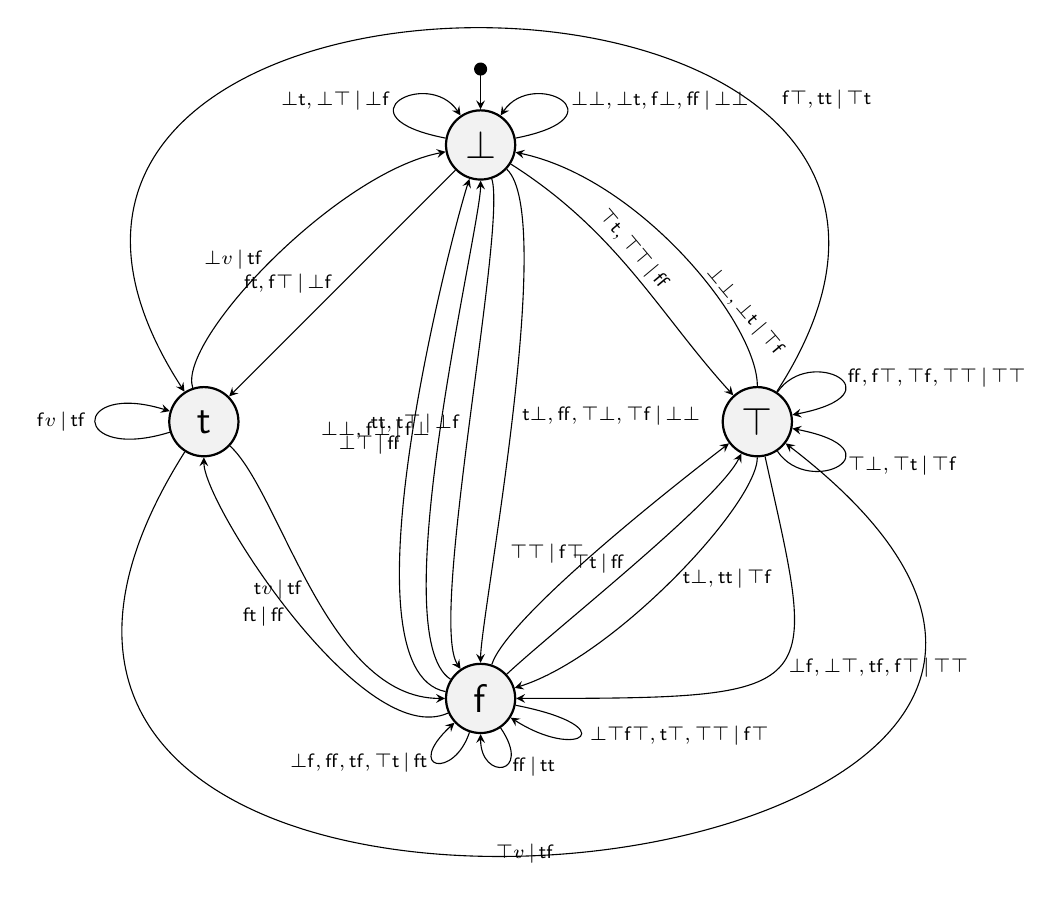
\begin{tikzpicture}[
        bezier bounding box=true,
        ->,
        >=stealth,
        node distance=0.25cm,
        every node/.style={font=\scriptsize},
        every state/.style={font=\Large, thick, fill=gray!10},
        initial text=$ $,
        initial distance=1.5cm,
        every initial by arrow/.style={*->},
        every edge/.append style={},
        yscale=-1,
        x=20pt,
        y=20pt
    ]
    \node[state, initial below] (bot) at (0,0) {\(\bot\)};
    \node[state] (true) at (-5,5) {\(\mathsf{t}\)};
    \node[state] (top) at (5,5) {\(\top\)};
    \node[state] (false) at (0,10) {\(\mathsf{f}\)};
    \draw (bot) edge[out=200, in=250, loop, distance=1.5cm] node[left]{
            \(\trs{\bot\mathsf{t},\bot\top}{\bot\mathsf{f}}\)
        } (bot);
    \draw (bot) edge[out=340, in=290, loop, distance=1.5cm] node[right]{
            \(\trs{\bot\bot,\bot\mathsf{t},\mathsf{f}\bot,\mathsf{f}\mathsf{f}}{\bot\bot}\)
        } (bot);
    \draw (bot) edge node[left]{
            \(\trs{\mathsf{f}\mathsf{t},\mathsf{f}\top}{\bot\mathsf{f}}\)
        } (true);
    \draw (bot) edge[out=45,in=240] node[near start, right, rotate=310, yshift=0.25cm]{
            \(\trs{\top\mathsf{t},\top\top}{\mathsf{f}\mathsf{f}}\)
        } (top);
    \draw (bot) edge[out=60, in=270, distance=1.5cm] node[right]{
            \(\trs{\mathsf{t}\bot,\mathsf{f}\mathsf{f},\top\bot,\top\mathsf{f}}{\bot\bot}\)
        } (false);
    \draw (bot) edge[out=80, in=250, distance=1.5cm] node[left]{
            \(\trs{\mathsf{t}\mathsf{t},\mathsf{t}\top}{\bot\mathsf{f}}\)
        } (false);
    \draw (true) edge[out=150, in=210, loop, distance=1.5cm] node[left]{
            \(\trs{\mathsf{f}v}{\mathsf{t}\mathsf{f}}\)
        } (true);
    \draw (true) edge[out=260, in=160, distance=1.5cm] node[left]{
            \(\trs{\bot v}{\mathsf{t}\mathsf{f}}\)
        } (bot);
    \draw (true) edge[out=60, in=180, distance=1.5cm] node[left]{
            \(\trs{\mathsf{t}v}{\mathsf{t}\mathsf{f}}\)
        } (false);
    \draw (true) edge[out=120,in=40,distance=10cm] node[left]{
            \(\trs{\top v}{\mathsf{t}\mathsf{f}}\)
        } (top);


    \draw (top) edge[out=290, in=340, loop, distance=1.5cm] node[right]{
            \(\trs{\mathsf{f}\mathsf{f},\mathsf{f}\top,\top\mathsf{f},\top\top}{\top\top}\)
        } (top);
    \draw (top) edge[out=70, in=20, loop, distance=1.5cm] node[right]{
            \(\trs{\top\bot,\top\mathsf{t}}{\top\mathsf{f}}\)
        } (top);
    \draw (top) edge[out=300,in=240,distance=8cm] node[near start,right,yshift=0.25cm]{
            \(\trs{\mathsf{f}\top,\mathsf{t}\mathsf{t}}{\top\mathsf{t}}\)
        } (true);
    \draw (top) edge[out=270,in=20,distance=1.7cm] node[near start, right, rotate=310,yshift=0.2cm,xshift=-0.9cm]{
            \(\trs{\bot\bot,\bot\mathsf{t}}{\top\mathsf{f}}\)
        } (bot);
    \draw (top) edge[out=80,in=0,distance=4cm] node[right]{
            \(\trs{\bot\mathsf{f},\bot\top,\mathsf{t}\mathsf{f},\mathsf{f}\top}{\top\top}\)
        } (false);
    \draw (top) edge[out=90,in=330,distance=1.5cm] node[right]{
            \(\trs{\mathsf{t}\bot,\mathsf{t}\mathsf{t}}{\top\mathsf{f}}\)
        } (false);

    \draw (false) edge[out=20, in=50, loop, distance=1.5cm] node[right]{
            \(\trs{\bot\top\mathsf{f}\top,\mathsf{t}\top,\top\top}{\mathsf{f}\top}\)
        } (false);
    \draw (false) edge[out=70, in=90, loop, distance=1.5cm] node[right]{
            \(\trs{\mathsf{f}\mathsf{f}}{\mathsf{t}\mathsf{t}}\)
        } (false);
    \draw (false) edge[out=100, in=120, loop, distance=1.5cm] node[left]{
            \(\trs{\bot\mathsf{f},\mathsf{f}\mathsf{f},\mathsf{t}\mathsf{f},\top\mathsf{t}}{\mathsf{f}\mathsf{t}}\)
        } (false);
    \draw (false) edge[out=140,in=90,distance=1.5cm] node[left]{
            \(\trs{\mathsf{f}\mathsf{t}}{\mathsf{f}\mathsf{f}}\)
        } (true);
    \draw (false) edge[out=230,in=90,distance=1.5cm] node[left]{
            \(\trs{\bot\bot,\mathsf{f}\bot}{\mathsf{f}\bot}\)
        } (bot);
    \draw (false) edge[out=200,in=100,distance=1.5cm] node[left]{
            \(\trs{\bot\top}{\mathsf{f}\mathsf{f}}\)
        } (bot);
    \draw (false) edge[out=300,in=105,distance=1.5cm] node[left]{
            \(\trs{\top\mathsf{t}}{\mathsf{f}\mathsf{f}}\)
        } (top);
    \draw (false) edge[out=280,in=125,distance=1.5cm] node[left]{
            \(\trs{\top\top}{\mathsf{f}\top}\)
        } (top);
\end{tikzpicture}
\end{document}